\chapter{Publishing microscopy data}

In this module, we will work through some necessary basics of image processing and explore common ways to visualize microscopy data. After this module, you should feel comfortable working with your images in Fiji and be able to use this knowledge to prepare your data for publication.

Digital images are ubiquitous and nearly everybody is used to taking pictures with a digital camera or smart-phone and also storing and processing these images. The same way that digital imaging has replaced analog cameras in our daily lives, light microscopes have transformed to digital imaging systems\footnote{In this course, we do not discuss the technologies that actually generate digital images in microscopes. If you want to learn about various microscopy techniques, we recommend looking at the online iBiology Microscopy Course (www.ibiology.org/ibioeducation/taking-courses/ibiology-microscopy-course.html, 25-02-2015)}. Even the most simple light microscopes are usually equipped with a digital camera and a screen to display, take and store images - also allowing quick and simple image processing tasks without the need for additional software (e.g. brightness \& contrast adjustments, white balancing). More complex light microscopes, such as confocal laser scanning microscopes (CLSM), already require sophisticated software interfaces to set up imaging parameters and visualize the results. Finally, there are also types of microscopes that depend on digital image processing (e.g. stochastic optical reconstruction microscope, STORM or single plane illumination microscopy, SPIM).

As a result of these advancements, modern digital microscopy offers more than just 'pretty pictures' - there are many imaging techniques that rely on computational analysis as well as methods for image enhancement, restoration and quantitative analysis. Modern microscopy cannot be understood without the basics of digital images and digital image processing. This knowledge is not only essential to make full use of the capabilities, but also to understand limitations -- a very important prerequisite to maintain scientific validity.

\minisec{Raster and vector images}
Typically, most pictures you work with (scanned documents, photos taken with a digital camera, pictures found on the web) are raster graphics (see Fig. \ref{fig:bitmap-graphics}). This means that these images are made up of a grid of \emph{pixels} (picture elements). Each pixel has a value that represents some property of the image (usually brightness). The range of this value is called \emph{bit-depth} and determines possible values at each pixel. Sometimes, the term \emph{bitmap image} is used for a raster image. For example, the image shown in figure \ref{fig:bitmap-graphics} illustrates a raster image with 420 x 420 pixels and a bit-depth of 1 byte. Therefore, we have a total of 176400 pixels, multiplied with 1 byte taking up a total of 172 kilobytes disc space. As you can see, the number of pixels and the bit-depth affect the required disc space. Additionally, we cannot easily change the size of the image; enlarging causes the image to look 'pixelated' or we have to use interpolation techniques to estimate the value of added pixels. Decreasing the number of pixels in the image might result in a loss of image features. There are plenty of commercial and open-source programs to work with raster images; representative software packages are Adobe Photoshop (Adobe Inc., San Jose) and GIMP (GNU Image Manipulation Program, The GIMP team, http://gimp.org).

\begin{figure}[!ht]
	\centering
		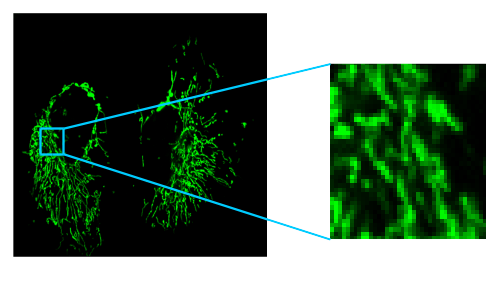
\includegraphics[width=0.60\textwidth]{mod1/figures/bitmap-graphics.png}
	\caption{Fluorescent labeled mitochondria in HeLa cells. THis image shows that raster graphics are made up of pixels that become clearly visible when zoomed.}
	\label{fig:bitmap-graphics}
\end{figure}


In contrast, vector graphics are not made up of a bitmap. Instead, they are based on geometrical shapes such as lines, curves, polygons or other shapes that are based on mathematical expressions. Therefore, these images can be scaled without a loss in image quality and typically use less disc space than raster images. Especially when the scaling of lines, text or other image content might change, it makes sense to use vector graphics (e.g. figures for a manuscript, scientific poster). Similar to the editors for raster images, there are plenty of vector graphics programs; representative examples are Adobe Illustrator (Adobe Inc., San Jose) and Inkscape (The Inkscape team, http://www.inkscape.org).

Often, programs support the conversion between raster and vector graphics. These are called \emph{rasterization} and \emph{vectorization}. Usually, vector graphics programs allow you to include raster-graphics without conversion.

Let's say you're done for the day and want to submit another great manuscript to Nature (Nature Publishing Group). Nature has detailed requirements on how your figures should be prepared for print (http://www.nature.com/nature/authors/gta/3c\_Final\_artwork.pdf, as of 08.10.2014). According to their guide, they prefer vector graphics for text and line-art. We will revisit the Nature figure requirements as we go along discussing properties of digital images!

\begin{verse}
\emph{Can you explain why journals prefer vector graphics for text and line-art?}
\end{verse}

\section{Pixels, spatial resolution and sampling frequency}
\label{sec:mod1-samplingrate}

It is important to remember that our microscopes have an optical resolution\footnote{For this course, we assume that you have a basic understanding why microscopes have an optical resolution and on which parameters the optical resolution depends.} that defines the ability to resolve details of the specimen. 

Limited by the optical resolution, the number of discrete pixels in a digital image then determines the spatial resolution. The number of pixels is usually called the sampling frequency (or sampling interval). This simply means that the spatial resolution depends on the number of pixels within given physical dimensions and that the maximum spatial resolution is limited by the optical resolution\footnote{This is only partially true -- we can theoretically build a microscope where the detector is the limiting factor. In general, the detector is chosen to match the optical resolution; and all internal microscope components involved in generating the digital image have to be matched as well.}. It is important to note that each pixel represents the average response of the optical system measured at a point within an area that is specified by the characteristics of our optical system. 

In a typical confocal microscope (not camera based), we can choose the number of pixels with which we want to sample the acquired image. A change in the pixel number obviously changes the size of the pixel and therefore also the area of which the average response is obtained. Choosing the wrong sampling frequency is a typical pitfall in microscopy, especially when zoom controls are used. If we sample inadequately, details can be lost. Oversampling is usually not critical, we just increase the amount of data we have to handle and we have to know that we oversample. Fortunately, sampling theory tells us exactly which sampling interval (pixel size, pixel number) is required to optimally represent the biological specimen given our optical resolution (the famous \emph{Nyquist theorem} states that we require a sampling interval $\geq$ twice the highest spatial frequency in our specimen and the highest frequencies we can observe are physically limited by our optical resolution). 

This raises the question why our microscopes even allow us to change the sampling frequency and not always simply operate at the diffraction-limited configuration. The reason is, that there are many experimental situations where it is desirable to intentionally lower our spatial resolution. Basically, we have to make a trade-off between the required resolution and imaging speed, amount of light collected at each pixel, photo-toxicity or other experimental parameters. The important thing is that we are aware of the fact that we under-sample for whatever reasons we have.

The limited number of discrete pixels in an image acquired with a microscope has serious consequences when you create figures for a manuscript. Publishers often require a certain number of pixels per cm (inch) to create high-quality figures and unfortunately, they leave it up to you to adjust your figures. However, they usually ignore the fact that you only have a limited number of pixels in your original data. One option you have is resampling your original data to change the number of pixels. Another option is to show pixels enlarged -- leading to a pixelated view of your data.

\subsection{Resampling Images}

Resampling an image changes the original data; the number of pixels is either increased or decreased (enlarging, shrinking). In comparison, using the zoom tool (icon magnifying glass) just increases or decreases the size of the pixels on your screen without resampling. Similar to other programs, Fiji also allows you to change the size of the canvas (the space on which your image is drawn, see Figure \ref{fig:adjust-canvas-dialog}. If you adjust the canvas size \texttt{[Image > Adjust > Canvas Size]}, the image is either cut (pixels outside the canvas size are cut off) or a margin is added where added pixels usually have the background color (zero value). 

\begin{figure}[!ht]
	\captionsetup{justification=centering}
	\centering
		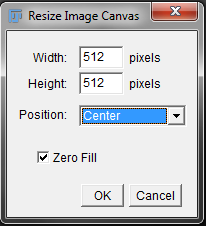
\includegraphics{mod1/figures/adjust-canvas-dialog.png}
		\caption{Adjust Canvas Size Dialog.}\label{fig:adjust-canvas-dialog}
\end{figure}

As you saw above, we determine the number of pixels during image acquisition according to our needs and the limits of the microscope. However, when you prepare your data for a presentation, poster or manuscript you will usually have to scale your original data. Before we discuss best practices and look at an example, we will introduce important basic terminology.

\minisec{Image resolution outside microscopy}

In printed images and in document scanners, resolution is often given in \emph{DPI (Dots Per Inch)}, the number of dots within a line that spans 1 inch (2.54 cm). Computer screen, tablet or phone resolution is typically given in \emph{PPI (Pixels Per Inch)}, the number of pixels within a line that spans 1 inch. Confusing, DPI is often used when PPI would be better, and even more confusing, one printer dot is usually not equal to one pixel! 

As we learned in section \ref{sec:mod1-samplingrate}, knowing the number of pixels is not sufficient to define the resolution -- pixel size (sampling rate, distance of pixels, ..) is necessary as well. This is also true for consumer products such as digital cameras, smartphones or flatscreen TVs. Knowing that a Full HD TV is capable of displaying 1920 x 1080 pixels presents no information about the size of each pixel. An 18 mega-pixel camera that is able to generate photos with 5184 x 3456 pixels also has no resolution associated. For screens, we can calculate the PPI by dividing the number of pixels by the size of the screen. For example, a 40'' Full HD TV would have 55.07 PPI, an IPhone 5 about 326 PPI (4'', 1640 x 1136 pixels but two dots per pixel!), an Amazon Kindle Paperwhite 212 PPI (6'', 1024 x 758). 

High quality photo printing requires about 200-300 PPI. With the number of pixels of our digital camera, we can calculate the maximum size of a high-quality print. For example, an 18 mega-pixel camera print with at least 200 PPI: 

\begin{quotation}
	18 mega-pixel = 5184 x 3456 pixels, divided by 200 PPI results in a print of about 65 x 43 cm (1 inch = 2.54 cm).
\end{quotation}

Publishers usually require that you submit your figures in 300-600 DPI (meaning PPI), depending on the content (e.g. see the requirements of Nature\footnote{http://www.nature.com/nature/authors/gta/3c\_Final\_artwork.pdf, as of 08.10.2014} or PNAS\footnote{http://www.pnas.org/site/misc/digitalart.pdf, as of 04/03/2015}). This already determines the maximum size of your (sub)figure given available pixels. 

\begin{taskbox}{Resampling Example - No Interpolation}

\begin{enumerate}
	\item Open the file resampling-test.tiff in /module1/data. This is a 20x20 pixel black-and-white (binary) image. Use the magnification tool to zoom to the maximum magnification. You should now see a one pixel wide and a two pixel wide vertical white line and a 1px diagonal line. 
	\item Before we perform image manipulations, we duplicate the original image for convenience \texttt{[Image > Duplicate]}.
	\item Go to [Image > Adjust > Size], you should see a dialog as shown in figure \ref{fig:adjust-size-dialog}.
	
	\begin{minipage}[t]{\linewidth}
		\begin{center}
		\adjustbox{valign=t}{%
			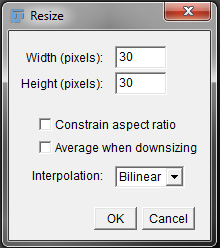
\includegraphics[width=0.3\textwidth]{mod1/figures/adjust-size-dialog.png}%
		}
		\medskip
		\captionof{figure}{Adjust Size Dialog.}\label{fig:adjust-size-dialog}
		\end{center}
	\end{minipage}
	
	\item Perform a resize to 30 x 30 pixels (150\% size), with no interpolation, and compare the result with the original figure. Use the \texttt{Line-Tool} (see fig. \ref{fig:line-tool}) to measure the width of both vertical lines. You should observe that one line was not scaled while the other was scaled to 150\%.
	
	\begin{minipage}[t]{\linewidth}
		\begin{center}
		\adjustbox{valign=t}{%
			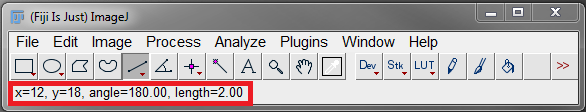
\includegraphics[width=0.7\textwidth]{mod1/figures/line-tool.png}%
		}
		\medskip
		\captionof{figure}{Line tool selection and values.}\label{fig:line-tool}
		\end{center}
	\end{minipage}
	
	\item Try other values for the resizing and observe the results.
\end{enumerate}

\end{taskbox}

\newpage
\begin{taskbox}{Resampling Example - With Interpolation}

\begin{enumerate}
	\item Again, work on a duplicate of the resampling-test.tif image.
	\item Adjust the size to 150\% with interpolation set to 'Bilinear'. Use the \texttt{Point-Tool} and move the mouse over the image. On the bottom of the Fiji bar, you should see the mouse position in pixels and the value of the current pixel (Figure \ref{fig:pixel-position}).
	
	\begin{minipage}[t]{\linewidth}
		\begin{center}
		\adjustbox{valign=t}{%
			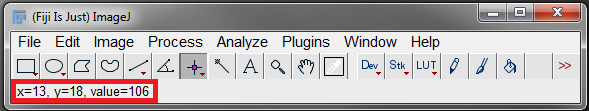
\includegraphics[width=0.7\textwidth]{mod1/figures/pixel-position.png}%
		}
		\medskip
		\captionof{figure}{Pixel position and value.}\label{fig:pixel-position}
		\end{center}
	\end{minipage}
	
	\item While the interpolation helps to visually estimate the 150\% re-sampling in the vertical and diagonal lines, you can see that the original data has been changed.
	\item Try other values for the resizing and observe the results.
\end{enumerate}
\end{taskbox}

As you should have observed, the bilinear interpolation leads to gray values appearing in the previously black-and-white image. Fiji supports the bilinear and the bicubic interpolation. Both interpolation algorithms sample pixel values surrounding each pixel to calculate the pixel value at the given position\footnote{For more information, Wikipedia has entries for bilinear and bicubic interpolations.}. 

Let us go back to our main question of making figures for a manuscript that we want to publish. PNAS recommends a minimum resolution of 300 DPI for color images and further suggests not to use interpolation when changing the size of the image. What should we do with our microscope images? Following guidelines should help you decide what to do:

\begin{itemize}
	\item Best practice: \emph{no image resampling ever} (e.g., see recommendations of the Journal of Cell Biology). Usually, you have enough pixels (>1000 x 1000 pixels), allowing you to choose an image size within your figure that is sufficient. For example, a 1000 x 1000 pixel image at 300 DPI results in about 130 pixels/cm -- you can choose a single column of 89 mm width (Nature requirements again) to display this image. If you then adjust the size of the image in your graphics software, you will only increase/decrease the size of each pixel (like the zoom tool) without resampling.
	\item Never resample more than once during image processing.
	\item Do the resampling at the end, after all other image manipulations and quantifications have been done.	
	\item Report any resampling procedures, including the original image size, pixel dimensions and the interpolation method.
	\item Most journals allow supplementary original data - a good way to present the raw, unfiltered data. Also, there is increasing interest to provide platforms that allow you to publish raw data (e.g. Figshare\footnote{www.figshare.com, an online digital repository - free to upload and free to access; as of 13.10.2014})
	\item Most important if you really have to resample: Convince yourself (and your lab-mates) that the original image and the re-sampled image convey the same information.
\end{itemize}

Fiji also has the option to directly interpolate the image to a given size and DPI (PPI!) using \texttt{[Image > Adjust > Scale To DPI]}. Using this function, you do not have to calculate the values yourself using the \texttt{[Adjust Size]} function (Fig. \ref{fig:scale-to-dpi-dialog}).
\begin{figure}[!h]
	\centering
		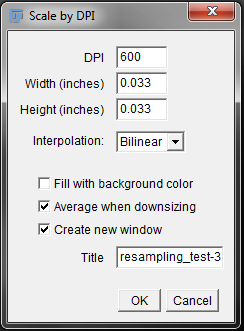
\includegraphics[width=0.3\textwidth]{mod1/figures/scale-to-dpi-dialog.png}
	\caption{Scale to DPI dialog.}
	\label{fig:scale-to-dpi-dialog}
\end{figure}

\newpage
\section{Bit-Depth \& Computer Number Representations}

We already introduced the term bit-depth that describes the range of values that can be represented at each pixel. When we refer to the possible values of each pixel, we use the terms brightness or intensity in the course context. It is very likely that you already encountered the words \emph{bit}, \emph{bits}, (kilo-, mega-, giga-)\emph{bytes} somewhere: 32/64-bit computers, 8/16-bit microscopy images or 50 Mbit/s internet connection speed.

A \emph{bit} is the elementary unit of binary numbers and its possible values are 0 and 1. Electronic devices code and store information with binary numbers because binary states (0 and 1) can easily be implemented in electronics\footnote{While this statement is true, it leaves out any details. However, there are plenty of resources on the web if you are really interested why and how bits are used.}. If you have two bits, you can represent 4 different states (00, 01, 10, 11). In general, if you have \textbf{n} bits, you can represent \textbf{2\textsuperscript{n}} different states. Therefore, 8 bits allow you to represent 256 (2\textsuperscript{8}) different brightness values and 16 bits already 65536 (2\textsuperscript{16}) different values. The higher the bit-depth of our image, the more gray-levels can be represented between black (0) and white (Maximum value). One \emph{byte} consists of 8 bits (historic and convenience reasons). One kilobyte is a multiple of a byte, either 1000 bytes or 1024 bytes; this can be confusing and usually depends on the context. The same is true for further multiples, such as mega-, giga-, tera-, and petabytes.

Similar to choosing an appropriate pixel size (see section \ref{sec:mod1-samplingrate}), we also have to make choices regarding the pixel intensity values during acquisition:
\begin{itemize}
	\item \emph{Bit-depth:} During image acquisition, we round the brightness values found in our samples into a certain number of levels that our chosen bit-depth can represent. For example, if we have 300 distinct brightness levels in our sample and we choose an 8-bit bit-depth, we cannot represent all 300 values (we only have 256 levels!). In this case, the 300 distinct values are rounded to the nearest level that can be represented. Pixels that have different intensities in our sample get rounded to the same values and the differences are lost. In practice, we do not worry about rounding errors during image acquisition -- we usually only have to make the choice between a low bit-depth (8-bit) and a higher bit-depth (12/16-bit). This is discussed in section \ref{sec:bitdepth-choice}. However, rounding errors can present problems during image processing. This is discussed in later chapters.
	\item \emph{Data saturation / clipping: } When you take images on a microscope, you usually set the laser output power, detector gain and detector offset for every image. The reason is that whatever bit-depth we chose, we want the brightest pixels just around the maximum value that can be represented by our bit-depth range and the darkest pixels just around zero. If we use the wrong settings and pixels are saturated/clipped, we loose information about the brightest and darkest parts of our sample. This can prevent further analysis of our data! Clipping can also occur during image processing as you will see in a few minutes.
\end{itemize}

The most common image bit-depths that you can generate with microscopes and that are supported in Fiji are:
\begin{itemize}
	\item 8-bit images that can display 256 gray levels with whole numbers (Integers).
	\item 16-bit images that can display 65536 different gray levels with whole numbers (Integers).
\end{itemize}

In addition, there is a 32-bit image format that allows you to display 2\textsuperscript{32} gray levels with real numbers. However, this format is a little bit more tricky to use as many functions in Fiji do not handle this bit-depth properly.

When you prepare your figures, bit-depth is usually not a big issue. However, you have to be careful when you export/import images using various file formats -- some common file formats only support 8-bit bit-depth and you have to make sure that you convert appropriately.

\newpage
\begin{taskbox}{Brightness Adjustments}
\begin{enumerate}
	\item Open the file fibroblast\_sim.tif in /data/chapter1. This is a 16-bit gray-scale image showing actin filaments in a cell. 
	\item You should note that the image looks rather dark. Fortunately, Fiji has a way to adjust the brightness and contrast of an image without altering the original data. Go to \texttt{[Image > Adjust > Brightness/Contrast...]}, you should see a dialog as shown in figure \ref{fig:adjust-brightness-dialog}.
	
	\begin{minipage}[t]{\linewidth}
		\begin{center}
		\adjustbox{valign=t}{%
			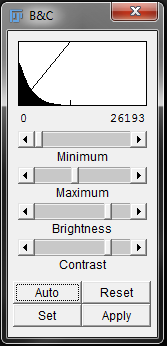
\includegraphics[width=0.3\textwidth]{mod1/figures/adjust-brightness-dialog.png}%
		}
		\medskip
		\captionof{figure}{Brightness and Contrast Adjustment.}\label{fig:adjust-brightness-dialog}
		\end{center}
	\end{minipage}
	
	\item Click on \texttt{[Auto]}. The image gets brighter as the maximum brightness is now associated with a lower image intensity. This linear scale can be adjusted manually by changing the slider positions. \texttt{[Reset]} reverts to the original intensity scaling. 
	\item Play with the sliders to set the image intensity scaling. 
	\item Using \texttt{[Set]}, we can either enter precise minimum and maximum values or show a defined range (8-,10-,12-,15-,16-bit) and also propagate our selection to all other open images. Again, the original pixel values remain, we only change the display.
\end{enumerate}

\end{taskbox}


\newpage
\begin{taskbox}{Bit-Depth Conversion}
\begin{enumerate}
	\item Open the image beads.tif from mod1/data using \texttt{[File > Open]}. Duplicate the image with \texttt{[Image > Duplicate...]}. Choose the line selection tool and draw a line through one of the bright spheres in the image (Fig. \ref{fig:line-roi-example}).	
	
	\begin{minipage}[t]{\linewidth}
		\begin{center}
		\adjustbox{valign=t}{%
			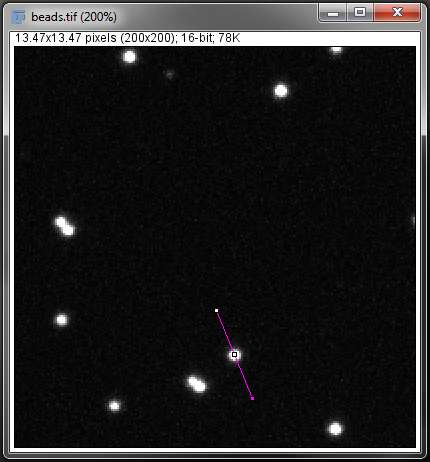
\includegraphics[width=0.5\textwidth]{mod1/figures/line-roi-example.png}%
		}
		\medskip
		\captionof{figure}{A line ROI through one of the beads.}\label{fig:line-roi-example}
		\end{center}
	\end{minipage}
	
	\item In the next step, we will look at the intensity (brightness) distribution along this line. For this, do \texttt{[Analyze > Plot Profile]} (Fig. \ref{fig:plot-profile-example}). You should observe that the gray value (y-axis) ranges from 0 to 65535 and that the curve looks cut at the upper end - this means that we have \emph{saturated} pixels, i.e. we cannot resolve any differences between these saturated pixels although the shape of the curve would suggest intensity changes. The [Plot Profile] function allows you to list (show), save and copy the values. If you click on \texttt{[Live]}, you can change the line ROI and the plotted profile will update. Try the update by drawing a line somewhere on the background and then again through a bead. Turn the live mode off again by another click on the button. 

\begin{minipage}[t]{\linewidth}
		\begin{center}
		\adjustbox{valign=t}{%
			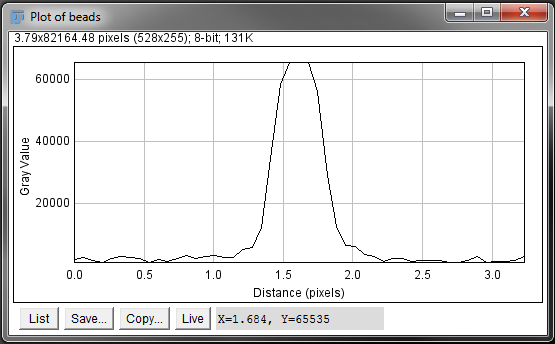
\includegraphics[width=0.5\textwidth]{mod1/figures/plot-profile-example.png}%
		}
		\medskip
		\captionof{figure}{Intensity profile of the line.}\label{fig:plot-profile-example}
		\end{center}
	\end{minipage}

\item Now, we convert the 16bit image to 8bit. First, we make sure that we scale during conversion by \texttt{[Edit > Option > Conversion]}. Then, we use \texttt{[Image > Type > 8-bit]} to convert the image. Make sure that the line ROI is still there and perform the plot profile function again. A second window pops up. Compare the plot profiles of the 8-bit and the 16-bit images. The conversion modified the brightness value (y-value). While the profiles are similar, the scaling is different. The image is scaled according to following equation:
	\[I_{8bit}=\frac{I_{16bit}(x,y)-min(I_{16bit}(x,y))}{max(I_{16bit}(x,y))-min(I_{16bit}(x,y))}*2^8
	\]
with:\\
I\textsubscript{16bit}(x,y): 16bit image\\
I\textsubscript{8bit}(x,y): 8bit image\\
max(I\textsubscript{16bit}(x,y)): maximum value of 16bit image\\
min(I\textsubscript{16bit}(x,y)): minimum value of 16bit image\\
\item Convert the image back to 16-bit and check the intensity values again. In this case, the intensity values are not increased. 
\item The conversion actually looks at the data as it is displayed. Adjust the brightness and contrast to an extreme value using \texttt{[Image > Adjust > Brightness/Contrast...]} (contrast slider to the right edge). Convert the image to 8-bit again. Look at the profile of a bead. You should see that the image only consists of 2 intensities: 0 and 255. As you saw, it is important to reset the brightness and contrast display before converting the image.
\end{enumerate}

\end{taskbox}

\subsection{Choice of Bitdepth}
\label{sec:bitdepth-choice}

The choice whether to use a low or high bit-depth depends on the application. Of course you could always use the maximum bit-depth available (to be on the safe side). However, this increases the amount of data you acquire. For example, going from 8-bit to 16-bit doubles the required harddisk space. In addition, image processing might be much slower as well! A typical application where a lower bit-depth is sufficient is where you have a very bright signal (signal-noise ration very good) and you just want to identify cells (vesicle, nuclei, ...) for counting or shape analysis. On the other hand, if you want to analyze bright regions as well as darker regions, or need precise intensity comparisons (e.g. for protein density measurements), a higher bit-depth is recommended.

\section{Image Dimensions}

Up to now, we just looked at 2-dimensional images, where each pixel \emph{p} can be identified by its spatial coordinates, its position along both axes \emph{p(x,y)}. In microscopy, we often deal with more dimensions, common scenarios are:

\begin{itemize}
	\item \textbf{3D z-stacks:} A single acquisition of a 3D volume. The additional dimension is the depth of the section. Each pixel \emph{p} can be identified by \emph{p(x,y,z)}.
	\item \textbf{3D time-series:} A sequence of 2D image acquisitions. The additional dimension is the time of the acquisition. Each pixel \emph{p} is identified by \emph{p(x,y,t)}. 
	\item \textbf{3D multi-channel images:} A 2D image is acquired with >1 color channel (multiple fluorophores). The additional dimension is the color. Each pixel is identified by \emph{p(x,y,c)}.
	\item \textbf{4D images:} a combination of 4 already discussed dimensions: z-stacks with multiple color channels, sequence of z-stacks over time or 2D multicolor image over time.
	\item \textbf{5D images:} a combination of all discussed dimensions: sequence of z-stacks with multiple color channels over time. Each pixel \emph{p} is identified by \emph{p(x,y,c,z,t)}.
\end{itemize}

Fiji allows you to work with all these image types and we will discuss those methods and possible ways to visualize these data in publications in the following sections.

\subsection{3D stacks}

For historical reasons, Fiji (ImageJ) has two different structures to handle 3D data. At first, ImageJ used \emph{stacks} to support 0-3 dimensions. This was done to z-slices or time points. To be more flexible, \emph{hyperstacks} were introduced to support 0-5 dimensions. For compatibility reasons, both structures co-exist at the moment, but the distinction is disappearing with the hyperstack becoming the standard structure to represent multi-dimensional data. As you will see, hyperstacks are used when importing microscopy file formats. If a pixel \emph{p} defined by three spatial dimensions \emph{p(x,y,z)}, we call the pixel \emph{voxel} (volume element).

\begin{taskbox}{Viewing a 3D Stack}

\begin{enumerate}
	\item Open the file flybrain-template.tif in /mod1/data. This is an 8-bit gray-scale z-stack, showing a standard template of a fly brain. You should see that there is a slider below the image to go through individual z-sections of the stack. 
	\item If the image looks too bright or dark, adjust the brightness (\texttt{[Image > Adjust > Brightness/Contrast...]}).
	\item Click on the start animation button left to the slider to start an automatic stepping through the sections (Fig. \ref{fig:stack_animation_button} similar to a video). Clicking on the button again, pauses the animation (button icon changes accordingly).
	
	\begin{minipage}[t]{\linewidth}
		\begin{center}
		\adjustbox{valign=t}{%
			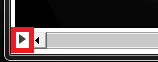
\includegraphics[width=0.3\textwidth]{mod1/figures/stack-animation-button.png}%
		}
		\medskip
		\captionof{figure}{Start stack animation.}\label{fig:stack-animation-button}
		\end{center}
	\end{minipage}
	
	\item Using the stack toolbar (Fig. \ref{fig:stack-toolbar}), you can \texttt{[Start Animation]} and \texttt{[Stop Animation]} as well.
	
	\begin{minipage}[t]{\linewidth}
		\begin{center}
		\adjustbox{valign=t}{%
			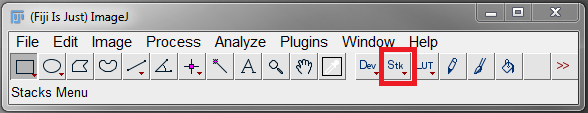
\includegraphics[width=0.7\textwidth]{mod1/figures/stack-toolbar.png}%
		}
		\medskip
		\captionof{figure}{Stacks toolbar.}\label{fig:stack-toolbar}
		\end{center}
	\end{minipage}
	
	\item Use the \texttt{[Animation Options]} from the stack toolbar to increase the animation speed to 20 fps (frames-per-second) and loop back and forth. The animation should look much smoother now (Fig. \ref{fig:animation-options-dialog}).
	
	\begin{minipage}[t]{\linewidth}
		\begin{center}
		\adjustbox{valign=t}{%
			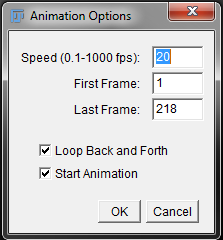
\includegraphics[width=0.4\textwidth]{mod1/figures/animation-options-dialog.png}%
		}
		\medskip
		\captionof{figure}{Stacks toolbar.}\label{fig:animation-options-dialog}
		\end{center}
	\end{minipage}
	
	\item When you want to use an animation of the stack in a presentation, you can save the stack as an avi using \texttt{[File > Save As > AVI...]}.
	
\end{enumerate}

\end{taskbox}

It is possible that the image data you import has the dimensions mixed up. If the data is a stack, you can use \texttt{[Image > Properties]} to reorder channels, slices and frames. However, it is more flexible to convert the stack to a hyperstack and perform re-ordering on the hyperstack.

\begin{taskbox}{Order of Dimensions}

\begin{enumerate}
	\item Open the file flybrain-template.tif in /mod1/data if it is not still open.
	\item Use \texttt{[Image > Hyperstacks > Stack to Hyperstack...]} to convert the stack to a hyperstack. In our test image, the order, channels, slices and frames should be detected correctly. 
	\item Now, you can easily re-order the dimensions of the hyperstack using \texttt{[Image > Hyperstacks > Re-order Hyperstacks...]}. Although this does not make any sense, change the z-dimension to a time dimension. As you can see, from the user perspective, this does not change anything at the moment.
\end{enumerate}

\end{taskbox}

Fiji offers many ways to manipulate (hyper)stacks. You can concatenate, combine, interleave, insert or split stacks; convert images to stacks and back, remove and add slices, make substacks, create a montage or generate a stack from a montage. These functions can be found under \texttt{[Image > Stacks]} and especially \texttt{[Image > Stacks > Tools]}. 

\begin{taskbox}{Manipulating Stacks -- Creating a Montage}
A common way 3-dimensional data is presented (typically along time or z-axis) is the montage view.

\begin{enumerate}
	\item Open the file flybrain-template.tif in /mod1/data if it is not still open.
	\item Use \texttt{[Image > Stacks > Make Montage...]}. In the dialog, set \texttt{[Columns]} and \texttt{[Rows]} to 5, \texttt{[First Slice]} to 100, \texttt{[Last Slice]} to 124, change the \texttt{[Border Width]} to 1 pixel and tick \texttt{[Label Slices]} (Fig. \ref{fig:make-montage-dialog}).
	
	\begin{minipage}[t]{\linewidth}
		\begin{center}
		\adjustbox{valign=t}{%
			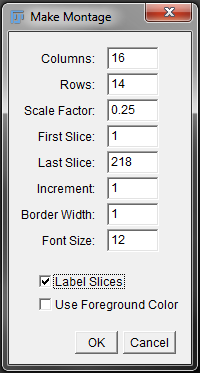
\includegraphics[width=0.4\textwidth]{mod1/figures/make-montage-dialog.png}%
		}
		\medskip
		\captionof{figure}{Make Montage Dialog.}\label{fig:make-montage-dialog}
		\end{center}
	\end{minipage}
	
	\item You can see how easy it is to create a custom montage view, play with the different options, e.g. \texttt{[Increment]}.
\end{enumerate}

\end{taskbox}

\begin{taskbox}{Manipulating Stacks -- Creating an Insert}
We now want to do something more complicated: let's say we want to show a detail of the flybrain, e.g. the central complex or the optic lobes. To help viewers, we want to put a little version of the complete brain in the corner of our 3D image as an overview. How would you proceed?

\begin{enumerate}
	\item Open the file flybrain-template.tif in /mod1/data if it is not still open.
	\item Use the rectangle tool to select an interesting part of the brain that you want to highlight. Duplicate the complete stack using \texttt{[Image > Duplicate]}, this will only duplicate the part you selected. 
	\item Use \texttt{[Image > Adjust > Size...]} to create an image with 1024 pixel width and no interpolation.
	\item Go back to our original image of the fly brain and use \texttt{[Image > Scale...]} to reduce the image size to 20\% (x, y) with bilinear interpolation.
	\item The insert is created with \texttt{[Image > Stacks > Tools > Insert...]}. Make sure you use the detailed view of brain as \texttt{[Destination]} and the overview as \texttt{[Source]}. \texttt{[X-Location]} and \texttt{[Y-Location]} can remain 0 (Fig. \ref{fig:stack-inserter-dialog}).
	
	\begin{minipage}[t]{\linewidth}
		\begin{center}
		\adjustbox{valign=t}{%
			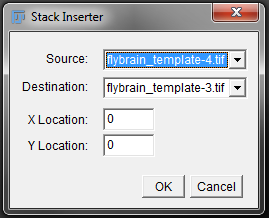
\includegraphics[width=0.4\textwidth]{mod1/figures/stack-inserter-dialog.png}%
		}
		\medskip
		\captionof{figure}{Stack Inserter Dialog.}\label{fig:stack-inserter-dialog}
		\end{center}
	\end{minipage}
	
	\item Again, a very easy procedure -- explore further stack operations on your own.
\end{enumerate}

\end{taskbox}

\subsection{Color images}

So far, we only analyzed images with one color channel (grayscale), i.e. at each spatial position, we only had one pixel with one value. In microscopy, we often encounter multi-channel images where each channel corresponds to one modality. One channel for each fluorophore intensity, a channel for a DIC image or even a channel that does not represent brightness but for example fluorophore lifetime. Outside microscopy, we also usually encounter color images, these are often RGB images that consist of red, green and blue 8-bit channels. Again, publisher demands on the color usage varies, sometimes they demand that the RGB color space you usually work with on your computer is converted to the CMYK color space that is typically used in print. Luckily, as the primary source for distributing and viewing a publication are various digital devices, conversion demands become less common. 

\minisec{Color models}
Outside microscopy, two colorspaces are very common:
\begin{enumerate}
	\item RGB (Red Green Blue)\\A single RGB image has three, fixed color channels: red, green and blue. Each of those have a fixed bit-depth of 8-bit, resulting in a single RGB image with 24-bit. These colors have been chosen as computer screens generate colors by mixing red, green and blue light and therefore, RGB images directly determine how much of each color to use but are device dependent (actually, RGB is based on human color perception).
	\item CMYK (Cyan Magenta Yellow Key)\\A single CMYK image is based on four colors: cyan, magenta, yellow and black. The color model is primarily used in printing, but is device-dependent as well. When you want to publish a manuscript, it is very likely that you will be asked to convert your figures to the CMYK color space. This can be done with Fiji using existing Plugins, but it might be better to perform the conversion for the total final figure when all other editing has been finished. As the online versions of publications have become much more important than the actual prints, efforts to produce color-true conversions for printing become much less important.
\end{enumerate}

\newpage
\begin{taskbox}{RGB Images}

\begin{enumerate}
	\item Open the file muscle-cell.tif in /mod1/data\. This image was taken from a publication in Nature Cell Biology 5, 598(2003); Cell of the Month: The vascular smooth muscle cell cytoskeleton; Mario Gimona; DOI:10.1038.ncb0703-598. This RGB image shows mouse smooth muscle cell with fluorescent labels of the cytoskeleton. Use \texttt{[Image > Show Info...]} for details about this image.
	\item Use \texttt{[Image > Adjust > Brightness/Contrast]} and change the slider values. Observe that this operation affects all colors simultaneously. Reset the changes.
	\item We now split the red, green and blue channels of the RGB image with \texttt{[Image > Color > Split Channels]}. Three windows appear, each showing the respective color content. 
	\item Let's combine these channels again with \texttt{[Image > Color > Merge Channels]}. The merge-function gives us many options to create a merged image (Fig. \ref{fig:merge_channels_dialog}). Do not set any options and use the same color channels.
	
	\begin{minipage}[t]{\linewidth}
		\begin{center}
		\adjustbox{valign=t}{%
			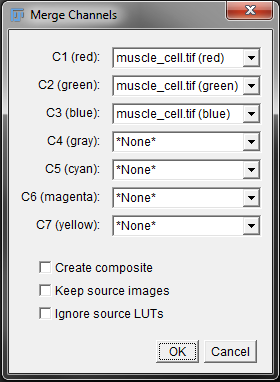
\includegraphics[width=0.4\textwidth]{mod1/figures/merge-channels-dialog.png}%
		}
		\medskip
		\captionof{figure}{Merge Channels Dialog.}\label{fig:merge-channels-dialog}
		\end{center}
	\end{minipage}
	
	\item Now split again and merge back, but with option \texttt{[Create composite]} ticked. This creates a slider below the image, indicating that we created a three-layered stack, one layer for each color.  
	\item The composite image allows us to work on each channel separately. Perform \texttt{[Image > Color > Channels Tool...]}. In this dialog, you can select individual channels in composite mode or view individual channels in Color/Grayscale mode (Fig. \ref{fig:channels-tool-dialog}). Try out the different settings.
	
		\begin{minipage}[t]{\linewidth}
		\begin{center}
		\adjustbox{valign=t}{%
			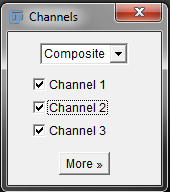
\includegraphics[width=0.4\textwidth]{mod1/figures/channels-tool-dialog.png}%
		}
		\medskip
		\captionof{figure}{Channels Tool Dialog.}\label{fig:channels-tool-dialog}
		\end{center}
	\end{minipage}
	
	\item Try to perform already know operations on just one color channel, e.g. Adjust the brightness (you can see that the little histogram changes color when you change the channel!).
\end{enumerate}

\end{taskbox}

\newpage
\begin{taskbox}{Convert RGB to CMYK -- Extending Fiji with Plugins}
Although Fiji has a great core functionality included, the power of this tool can only be appreciated with the many existing macros and plugins. While some plugins are already included in the Fiji distribution, you most likely will encounter some function you need that is not included -- and if this is a common task it is very likely that someone already solved this problem. 

\begin{enumerate}
	\item Convert the composite image back to a RGB image with \texttt{[Image > Color > Stack to RGB]}.
	\item We now want to convert the RGB image into a CMYK image for publication. However, Fiji is not able to do so and we have to extend the functionality. A quick search ('imagej convert to cmyk') shows that, fortunately, Stephan Saalfeld and Wayne Rasband wrote a plugin for this (two names you might encounter more often).
	\item You can find the file RGB\_to\_CMYK.class in the folder mod1/data/. Installing this plugin is very easy, just drag and drop the file onto the main Fiji window. You are asked to save the file in the plugins directory of Fiji. 
	\item Convert the image to CMYK with \texttt{[Plugins > RGB to CMYK]}.
\end{enumerate}

\end{taskbox}

\minisec{Lookup Tables}
For a computer, an image is a matrix with the same dimensions as the image and the range of possible values at each matrix position are determined by the bit-depth. A \emph{lookup table (LUT)} maps these values to a color/brightness that is displayed on the screen. Often, the LUT is simply called \emph{colormap}. The default LUT is gray-scale that, in an 8-bit image, assigns black to zero and white to 255. Intermediate values are represented as gray-levels and the same idea applies to any bit-depth.
The advantage using a LUT is obvious; we can create arbitrary LUTs with any coloring we want. These colored LUTs are called 'pseudo-color'. These LUTs are typically used to indicate fluorophore emission wavelengths but are sometimes changed to emphasize certain aspects of the data.

Figure \ref{fig:lookup-tables} shows the LUTs available in Fiji, the figure was created by the command \texttt{[Image > Color > Display LUTs]}. Very common LUTs are \emph{grayscale}, \emph{spectrum}, \emph{fire} and \emph{physics}.

\begin{taskbox}{Exploring Lookup Tables}

\begin{enumerate}
	\item Open the image beads.tif in /mod1/data. You can look at the LUT of the current image with \texttt{[Image > Color > Show LUT]} which is the standard linear grayscale LUT you have already seen.
	\item Change the LUT using \texttt{[Image > Color > Edit LUT...]}. Click on the top-left dark value and change the color from black to blue,  select the white entry from the bottom right and change the color to red (Fig. \ref{fig:lut-editor}).
	
	\begin{minipage}[t]{\linewidth}
		\begin{center}
		\adjustbox{valign=t}{%
			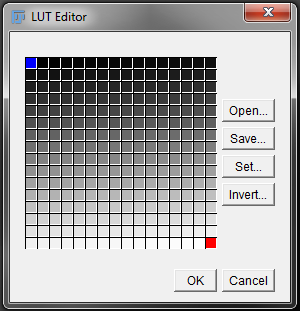
\includegraphics[width=0.4\textwidth]{mod1/figures/lut-editor.png}%
		}
		\medskip
		\captionof{figure}{LUT Editor.}\label{fig:lut-editor}
		\end{center}
	\end{minipage}
	
	\item Look at the image. Does it look familiar? This is the HiLo LUT that is often used in microscopy to optimize parameters for acquisition (emitted light, gain, offset). You can obtain the same image by selecting the HiLo LUT in Fiji (Fig. \ref{fig:lut-tool}).
	
	\begin{minipage}[t]{\linewidth}
		\begin{center}
		\adjustbox{valign=t}{%
			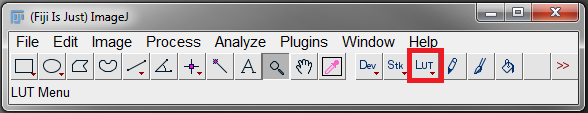
\includegraphics[width=0.4\textwidth]{mod1/figures/lut-tool.png}%
		}
		\medskip
		\captionof{figure}{LUT Tool.}\label{fig:lut-tool}
		\end{center}
	\end{minipage}
	
	\item Close the image and open the file cell-colony.tif in /mod1/data. Change the LUT to Spectrum using \texttt{[Image > Lookup Tables > Spectrum]}.
	\item Display the current LUT of the image. Try out different available LUTs and display their profile.
\end{enumerate}

\end{taskbox}

\begin{figure}[!ht]
	\centering
		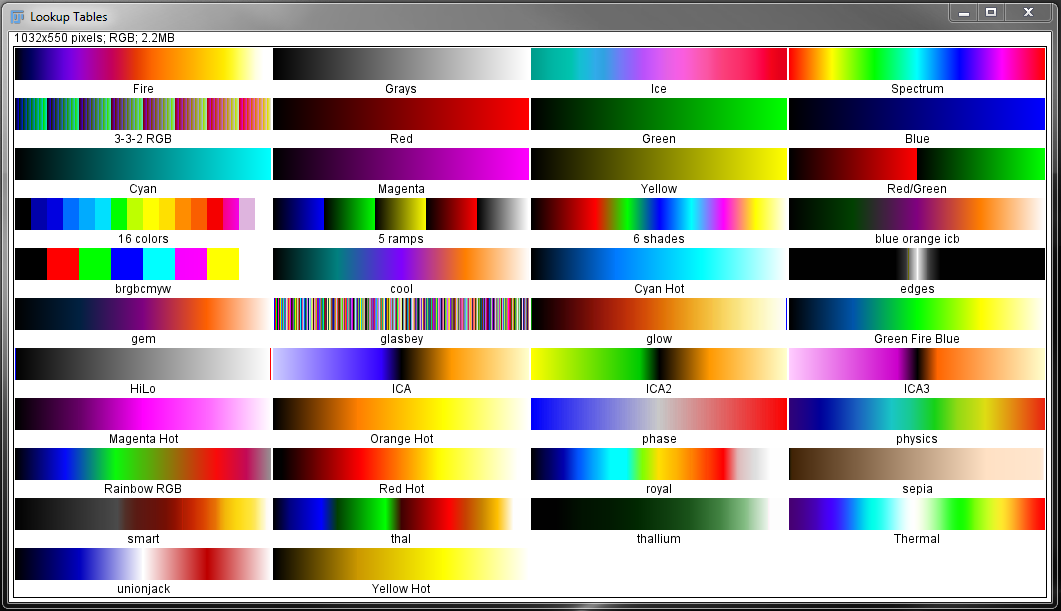
\includegraphics[width=0.80\textwidth]{mod1/figures/lookup-tables.png}
	\caption{Lookup Tables in Fiji}
	\label{fig:lookup-tables}
\end{figure}

\minisec{A short note about colors in publications}
There is plenty of literature around discussing the best colormaps and general rules one should apply when using colors in scientific publications. We do not want to enter this, sometimes heated, debate, as color choice in microscopy usually comes naturally based on the wavelengths. Nevertheless, we want you to get a feeling why this debate is going on and provide two examples: \emph{Color Bias} and \emph{Color Blindness}. Color bias refers to the problem that poor color choices can introduce a biased view of our data. For example, when we change the grayscale LUT to a spectrum LUT, relative changes of intensity can be obscured. Color blindness addresses the issue that microscopy images, especially illustrating colocalization, are often presented with red and green (all following information on color blindness is taken from \cite{wong2011}). However, a substantial number of people are affected by various forms of color blindness (about 8\% of male Europeans). Therefore, it is very likely that you will have reviewers for your manuscripts or audience in your talk that are color blind. One option to adjust your images is simply to replace the red with magenta.

\newpage
\begin{taskbox}{Effects of LUT Changes}

\begin{enumerate}
	\item Open the image muscle-cell.tif in /mod1/data. 
	\item Simulate color-blindness with \texttt{[Image > Color > Simulate Color Blindness]}. This function only works on an RGB image. 
	\item Use \texttt{[Image > Color > Replace Red with Magenta]} to exchange colors and then simulate color-blindness again. Color differences are much more obvious in the second image.
	\item go back to the original image of the muscle and split the channels.
	\item Duplicate the window containing the blue channel information.
	\item Change the LUT to spectrum and discuss the differences between the gray and spectrum LUTs.
\end{enumerate}

\end{taskbox}


\newpage
\begin{taskbox}{Calibration Bars}
A calibration bar is typically added to a figure when intensity comparisons are made. A calibration bar indicates which color corresponds to which brightness. This is especially important when you use LUTs with more than one color or when you use a single color LUT where the change in intensity is not linear ('gamma').

\begin{enumerate}
	\item Open the image fibroblast-sim.tif in /mod1/data. 
	\item Adjust Brightness/Contrast and select a LUT you like.
	\item Add a calibration bar with [Analyze > Tools > Calibration Bar...]. In the dialog, choose a location, fill color, label color, number of labels, asf. (Fig. \ref{fig:calibration-bar-dialog}). Note that this calibration bar shows the brightness settings you just applied and that you cannot change those now.	
	
	\begin{minipage}[t]{\linewidth}
		\begin{center}
		\adjustbox{valign=t}{%
			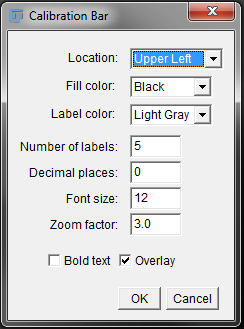
\includegraphics[width=0.4\textwidth]{mod1/figures/calibration-bar-dialog.png}%
		}
		\medskip
		\captionof{figure}{Calibration Bar Dialog.}\label{fig:calibration-bar-dialog}
		\end{center}
	\end{minipage}
	
\end{enumerate}

\end{taskbox}

\subsection{4D/5D stacks}
It is common that the data you acquire on microscopes has more than 3 dimensions. In this section, we will first discuss how you work with these data before we will discuss the problem of presenting this data in a figure.

With the hyperstack data format, representation of 4D and 5D data is very similar. Basically, sliders are added to the image window. However, you have to keep the order of dimensions in mind. Common dimension order is XYCZT, however this order might be different when you import data -- doublecheck when importing!

\begin{taskbox}{Working with 5D Data}
To illustrate working with 5D data, we will import a sequence of files that are labeled with \_t000\_z000\_c000 and increasing numbering. The sequence of files has been generated from the standard Fiji sample Mitosis \texttt{[File > Open Samples > Mitosis (26 MB, 5D stack)]}. This data shows Drosophila S2 cell expressing GFP-Aurora B and mCherry-tubulin fusion protein undergoing mitosis (Courtesy of Eric Griffis).

\begin{enumerate}
	\item Go to \texttt{[Plugins > Bio-Formats > Bio-Formats Importer]} and select the first image in the folder /mod1/data/mitosis.
	\item The Bio-Formats import options dialog shows up, make sure to select [Group files with similar names].
	\item In the dialog, you can choose how to stitch the files (Fig. \ref{fig:bioformats-file-stitching}). We select Pattern. This parses the file based on: mitosis\_t0<01-51>\_z00<1-5>\_c00<1-2>.tif. <> denote the range of the import, e.g. we could only select one channel, or any other substack.
	
	\begin{minipage}[t]{\linewidth}
		\begin{center}
		\adjustbox{valign=t}{%
			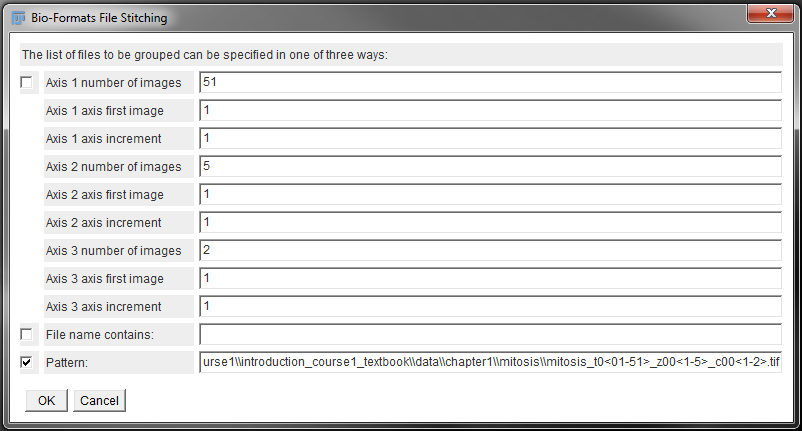
\includegraphics[width=0.8\textwidth]{mod1/figures/bioformats-file-stitching.png}%
		}
		\medskip
		\captionof{figure}{Bio-Formats File Stitching Dialog.}\label{fig:bioformats-file-stitching}
		\end{center}
	\end{minipage}
	
	\item The imported image shows three sliders: channel (2), z-position(5), time-stamps(51). Browse through the image, adjust Brightness if necessary. On thing to notice is that we lost information about the z-spacing, distance between time-stamps or channel colors.
\end{enumerate}

\end{taskbox}

\subsection{Visualizing Multidimensional Data}
You already worked with the most basic visualization of multidimensional data that only displays two dimensions at a time. In this view, you can browse through the dimensions by adjusting the sliders. Another view we already discussed is the image montage. Both of these visualizations are also valid options to present the data in a figure. In general, visualizing multi-dimensional data is non-trivial, as we are constrained by the physical limitations of our visual sense. In this section, we will look at some common visualization techniques for multi-dimensional microscopy data that are useful to highlight certain aspects of your data in a figure.

\begin{taskbox}{Projection (Dimensionality reduction)}
The first visualization we will explore is the projection. In a projection, data is summarized along one axis (dimension). A typical case is the maximum intensity projection of the z-axis of a 3D stack, resulting in a 2D image where each pixel represents the maximum value that was found in this \emph{(x,y)} position along \emph{z} - which is then used for the manuscript. In Fiji, you can choose between the minimum, average or maximum intensity projection and the sum, standard deviation or median of each pixel along \emph{z}. Remember that you can swap dimensions with \texttt{[Image > Hyperstack > Re-order Hyperstack]}.

\begin{enumerate}
	\item Open the image GMR-10A12-AE-01.tif from /mod1/data. This image shows the expression patterns of a GAL4 line, displayed on a standardized fly brain template (credits belong to the Rubin-lab, JFRC (Arnim Jennet) and The Virtual Fly Brain). Try to estimate the expression pattern (green) by going through \emph{z} using the slider. 
	\item In this case, we might decide a z-projection is helpful to quickly determine whether the expression pattern is of interest. We can perform the projection with \texttt{[Image > Stacks > Z Project...]}, choosing Max Intensity (Fig. \ref{fig:z-projection-dialog}).
	
	\begin{minipage}[t]{\linewidth}
		\begin{center}
		\adjustbox{valign=t}{%
			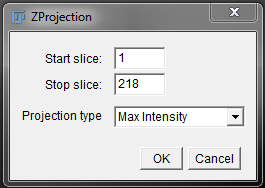
\includegraphics[width=0.4\textwidth]{mod1/figures/z-projection-dialog.png}%
		}
		\medskip
		\captionof{figure}{Z Projection Dialog.}\label{fig:z-projection-dialog}
		\end{center}
	\end{minipage}
	
	\item Explore various projections on the stack created from the file sequence in mod1/data/mitosis/.
\end{enumerate}

\end{taskbox}

\begin{taskbox}{Orthogonal View}
Another very common visualization is the orthogonal view. In this view, two additional windows are created that are linked to the current slider position of the 2D view. These windows show the XZ and YZ position. This visualization can be useful if you want to present the intensity profiles in 3D data while presenting overview images for the orientation of the reader at the same time.

\begin{enumerate}
	\item Open the stack GMR-10A12-AE-01.tif from mod1/data/ if it is not already open. Show the orthogonal view with \texttt{[Image > Stacks > Orthogonal Views]}. Try scrolling through the axes to get a feeling for this view.
\end{enumerate}

\end{taskbox}

\newpage
\begin{taskbox}{Color Coding}
One option to add a third dimension on a 2-dimensional plot is to somehow code the information; e.g. using different colors for z-depth or time. This can be useful when the data is structured along on axis, e.g. different layers of cells within a tissue, axons growing into other tissue parts or vesicles moving around over time.

\begin{enumerate}
	\item Open the image fake-tracks.tif from /mod1/data (another Fiji sample image). We use a fake file to better illustrate how the color coding works, but you can apply it to any 3D data for further testing. Perform [Image > Hyperstacks > Temporal-Color Code] and select a LUT of your choice (Fig. \ref{fig:color-code-dialog}).
	
	\begin{minipage}[t]{\linewidth}
		\begin{center}
		\adjustbox{valign=t}{%
			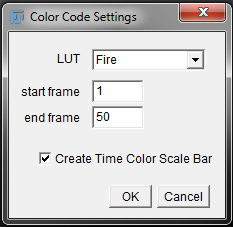
\includegraphics[width=0.4\textwidth]{mod1/figures/color-code-dialog.png}%
		}
		\medskip
		\captionof{figure}{Temporal Color Code Dialog.}\label{fig:color-code-dialog}
		\end{center}
	\end{minipage}
	
	\item Compare the color-coded image with the original time-series.
\end{enumerate}

\end{taskbox}

\begin{taskbox}{Generating a Kymograph Plot}
A Kymograph is an visualization to present a dynamic process in a single image where movements along a line are plotted for all time-frames in a stack (\emph{x-t} plot). Therefore, it is also a way to deruce dimensionality. They are common to show cellular components moving along a some path (e.g. mitochondria moving along an axon or cells migrating in reference to a body axis during development).

\begin{enumerate}
	\item Open the stack axon-mitos.tif from /mod1/data (Image by Arun Akondadi, Rugarli Lab, University of Cologne). Adjust Brightness. This image shows mitochondria moving along an axon.
	\item This image has a problem: the axon was not stained itself, but we can hopefully reconstruct the axon path by the positions of the moving mitochondria. For this, perform a maximum projection over time.
	\item The maximum-intensity image helps a lot to estimate the axon position in the image. Right-click on the [Line-Tool] to change the Straight Line to a Segmented Line (Fig. \ref{fig:segmented-line-selection}). Use the segmented line to trace the axon path. A double-click ends the line.	
	
	\begin{minipage}[t]{\linewidth}
		\begin{center}
		\adjustbox{valign=t}{%
			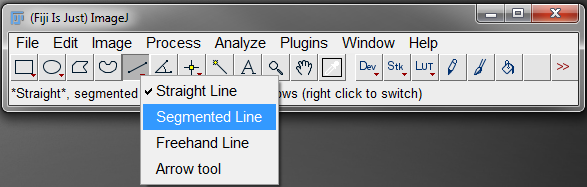
\includegraphics[width=0.6\textwidth]{mod1/figures/segmented-line-selection.png}%
		}
		\medskip
		\captionof{figure}{Segmented Line Tool.}\label{fig:segmented-line-selection}
		\end{center}
	\end{minipage}
	
	\item Go to the original stack and do \texttt{[Edit > Selection > Restore Selection]}. This restores the line we just selected on the maximum projection on the stack.
	\item Use \texttt{[Image > Stack > Reslice]} to generate the Kymograph. For display reasons, you can also invert the image with \texttt{[Edit > Invert]} and Adjust the Brightness.
	\item If the line was placed correctly, you should see something similar to Fig. \ref{fig:kymograph}. The kymograph helps to distinguish stationary mitochondria and we can sometimes even distinguish anterograde from retrograde movement (in reference to soma).	
	
	\begin{minipage}[t]{\linewidth}
		\begin{center}
		\adjustbox{valign=t}{%
			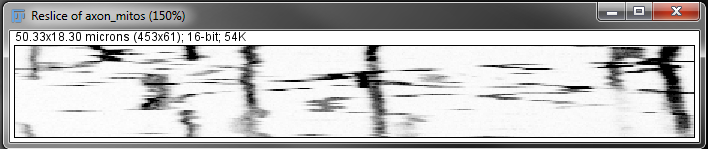
\includegraphics[width=0.6\textwidth]{mod1/figures/kymograph.png}%
		}
		\medskip
		\captionof{figure}{Example Kymograph.}\label{fig:kymograph}
		\end{center}
	\end{minipage}
	
\end{enumerate}

\end{taskbox}

\newpage
\begin{taskbox}{3D View}
Instead of trying to visualize our data in 2 dimensions, we can also visualize in 3D using the 3D viewer in Fiji. For visualizations in 3D, several display options are common: Volume, Orthoslice, and Surface. While this choice is obviously not available for printed figures, online publishing of supplementary videos can be a good option to present your data.

\begin{enumerate}
	\item Open the stack GMR-10A12-AE-01.tif from /mod1/data if it is not already open. Select the 3D viewer with [Plugins > 3D Viewer]. In the options dialog (Fig. \ref{fig:3D-viewer-dialog}), select the image and display as a volume.	
	
	\begin{minipage}[t]{\linewidth}
		\begin{center}
		\adjustbox{valign=t}{%
			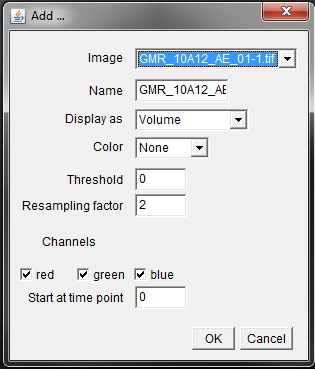
\includegraphics[width=0.3\textwidth]{mod1/figures/3D-viewer-dialog.png}%
		}
		\medskip
		\captionof{figure}{3D Viewer Dialog.}\label{fig:3D-viewer-dialog}
		\end{center}
	\end{minipage}
	
	\item Depending on your hardware, this might take a while to display. Try to navigate the 3D view with your mouse. 
	\item Let us try to generate a movie that you can save as an avi file. Use the 3D viewer menu to create a simple 360 degree rotation with \texttt{[View > Record 360 degree rotation]}. This generate a stack that you can now save as a movie using \texttt{[File > Save As > AVI]}. In this dialog, you can set the compression as well as the frame rate (how fast the movie is displayed). For our purposes, we set the compression to uncompressed and the Frame Rate to 15 fps (frames-per-second). Movie generation for journals can also be a tricky thing as they often impose strict size limits and requires specific formats. You often need to adjust the movie size as well as the compression algorithm to adhere to these requirements and the choice of both can be complicated. However, you can usually accept some compression artefacts as movies are often not considered raw data but more of a nice additional visualization. Still, make sure that you adhere to scientific principles and tell specifically how you treated your data to generate the movie.
	\item Further instructions on the 3D viewer can be found at: http://3dviewer.neurofly.de/; the website of the developers (as of 28.10.2014).
\end{enumerate}

\end{taskbox}

\section{File Formats}
File formats are an important, but dry topic. Every time you share data with colleagues or during the manuscript submission process, you have to work with various formats. This section discusses some basics of formats, focusing on formats suitable for microscopy data (and more general image file formats).

An image file consists of two main parts:
\begin{enumerate}
	\item \emph{Header} -- The header contains additional information about your image, such as image type, dimensions, bit-depth, pixel size, microscope settings and general file information. The data in the header is often called \emph{metadata}. Parts of the metadata are as important as the pixel data as they are necessary to interpret the image data (e.g. pixel size, bit-depth). 
	\item \emph{Content} -- The content of an image file consists of the actual pixel data, the matrix with numerical values. 
\end{enumerate}

The way the header and the pixel data are organized is determined by the file format. Many general image file formats exists, common are JPEG, PNG, TIFF or GIF. These formats are read by many different software tools across platforms and allow quick previews in all major operating systems. They are therefore very suitable to view and share image data. However, there are some problems with these file formats when we want to use them to store our scientific image data:
\begin{itemize}
	\item The format \emph{metadata} might not include essential information about our microscopy data (e.g. pixel size).
	\item \emph{Bit-depth} choice can be limited (e.g. GIF only allows 8-bit).
	\item \emph{Multi-dimensional information} might not be supported and extra-dimensions lost when converted (limits apply to all standard formats).
	\item The format uses \emph{lossy compression} to shrink file size (e.g. JPEG).
	\item Sometimes, limits on the \emph{maximum number of pixels} in a plane can prevent use for microscopy data.
\end{itemize}

\minisec{Compression}
Compression is used to reduce image file sizes. In general, compression methods can be divided into two types: \emph{loss-less} and \emph{lossy} compression. As the names indicate, the original pixel data cannot be reconstructed if lossy compression is employed (information is lost) and the original data can be reconstructed in lossless compression. A typical example of lossless compression is used in PNG. In this format, compression is achieved by shrinking redundant parts. JPEG and GIF are usually lossy formats. In addition to shrinking redundant parts, these formats also interpolate parts of the image to decrease file size even more.  

\begin{quotation}
	Lossy compression should be avoided to maintain scientific integrity!\\(Unless you know exactly what you are doing)
\end{quotation}

Limitations of general image file formats led many microscope and image processing software manufacturers to develop their own image file formats (LIF, SCN -- Leica, LSM, ZVI -- Zeiss, ND2 -- Nikon, ...). These formats store all important metadata information and the original pixel data (only loss-less compression used). However, the drawback is that you typically need proprietary software to view these files and access all metadata and that another software you want to use for analysis or display might not be able to read the original data file.

\begin{quotation}
	The originally acquired files are the most trustworthy -- this is your original, raw data\\You should always keep these files with appropriate backup solutions\footnote{It is also very likely that the funding agency supporting your research has rules how you treat your original data!}.
\end{quotation}

As you can see, this is a mess for researchers. On the one hand, you want to maintain scientific integrity and adhere to standards concerning your data, but on the other hand, you want to share your data and have easy access for further processing.

Fortunately, the LOCI Bioformats plugin\footnote{http://www.openmicroscopy.org/site/support/bio-formats5/ (as of 24/10/2014)} can import most proprietary file formats and extract most of their metadata in Fiji. There is also significant effort by the Open Microscopy Environment (OME) to provide a standardized file format OME-TIFF that includes rich metadata descriptions suitable for microscopy. This is an ongoing process and if you use this format to store and share data, you have to make sure that all important metadata is actually included.

Journals usually accept common image file formats (if compressed with loss-less compression). I would recommend using a vector graphics program for final figure preparation (think about text/line art) with microscopy images embedded (that have been prepared by e.g. Fiji).

\begin{taskbox}{Using Bioformats}
Let's import a microscope specific file format into Fiji.

\begin{enumerate}
	\item Open the image sted-confocal.lif in /mod1/data by drag/drop or with \texttt{[Plugins > Bio-Formats > Bio-Formats Importer]}.  
	\item In the next dialog, you can select various import options (Fig. \ref{fig:bioformats-import-dialog}). Make sure that you load the data into a Hyperstack and tick the Display metadata option.
	
	\begin{minipage}[t]{\linewidth}
		\begin{center}
		\adjustbox{valign=t}{%
			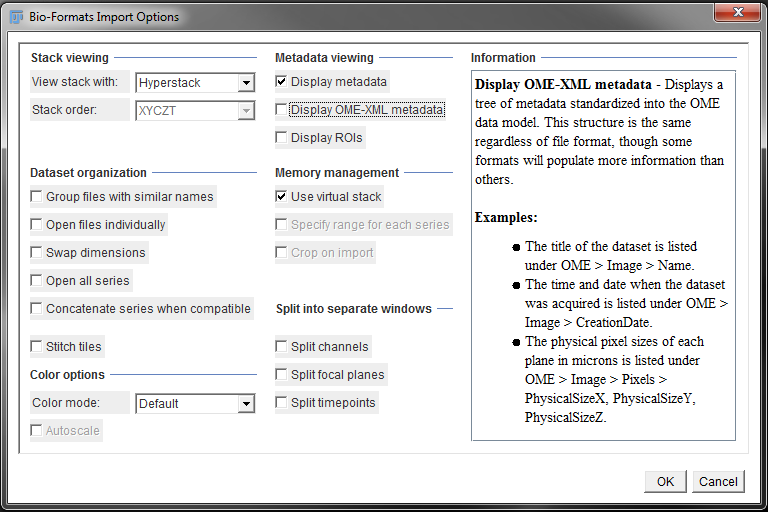
\includegraphics[width=0.8\textwidth]{mod1/figures/bioformats-import-dialog.png}%
		}
		\medskip
		\captionof{figure}{Bioformats Import Dialog.}\label{fig:bioformats-import-dialog}
		\end{center}
	\end{minipage}
	
	\item The next window allows you to select a series. Several microscope image formats are actually libraries of files. In this case, you should see three different files. Open one of the series.
	\item Two windows are opened. One showing the image, the other showing the metadata information. Scroll through the information and find the Dimension Length, Number of Elements and Unit. Use these values to calculate the pixel size.
\end{enumerate}

\end{taskbox}

\begin{taskbox}{Scale Bars}
Let's explore one final thing you usually have to include in your microscopy data: a scale bar that indicates the size of each pixel.

\begin{enumerate}
	\item Open the image sted-confocal.lif in /mod1/data by drag/drop or with \texttt{[Plugins > Bio-Formats > Bio-Formats Importer]}.  
	\item We now want to add a scale bar to our image. In this case, Fiji already knows the pixel size - let us check whether our previous calculations were correct. Go to \texttt{[Analyze > Set Scale...]}. This dialog should show you how many pixels are in one micrometer (Fig. \ref{fig:set-scale-dialog}).
	
	\begin{minipage}[t]{\linewidth}
		\begin{center}
		\adjustbox{valign=t}{%
			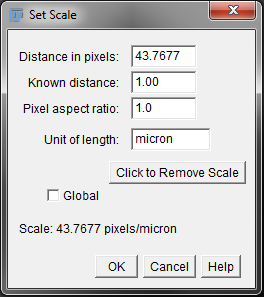
\includegraphics[width=0.4\textwidth]{mod1/figures/set-scale-dialog.png}%
		}
		\medskip
		\captionof{figure}{Set Scale Dialog.}\label{fig:set-scale-dialog}
		\end{center}
	\end{minipage}
	
	\item In case you have an image where information about the scale is visible in the image itself, you can then measure the length with a line and include this information in the dialog. Clicking on Global helps if you take one image of a micro-scale and want to use this information in other images you took with the same settings (e.g. on a small Lab-Microscope).
	\item Let's add a scale bar now. Use [Analyze > Tools > Scale Bar]. Similar to the calibration bar, the dialog lets you adjust various visual parameters (Fig. \ref{fig:scale-bar-dialog}).
	
	\begin{minipage}[t]{\linewidth}
		\begin{center}
		\adjustbox{valign=t}{%
			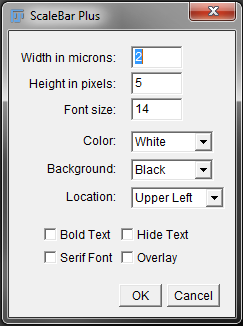
\includegraphics[width=0.4\textwidth]{mod1/figures/scale-bar-dialog.png}%
		}
		\medskip
		\captionof{figure}{Scalebar Dialog.}\label{fig:scale-bar-dialog}
		\end{center}
	\end{minipage}
	
\end{enumerate}

\end{taskbox}

\section{Figure publishing plugins for Fiji}
If you want to generate your figures completely in Fiji, there are great (published) plugins available that help you with this task (http://fiji.sc/2013-11-04\_-\_Plugins\_for\_making\_scientific\_Figures. as of 25/02/2015). The FigureJ plugin lets you specify a figure canvas on which you can place various images with labels and scale bars (http://imagejdocu.tudor.lu/doku.php?id=plugin:utilities:figurej:start, as of 25/02/2015).

